% chapters/methodology.tex
\chapter{Methodology}
\label{ch:methodology}

This chapter describes the three-stage evaluation framework developed to address the
two research aims. The pipeline is illustrated in Figure~\ref{fig:pipeline} and
consists of: (A) defining and weighting evaluation criteria via AHP, (B) selecting
discriminative questions from the MMLU Economics dataset, and (C) aggregating Likert
ratings through interval-based representations. Each stage is described below,
together with its implementation in the accompanying Python notebooks.

\begin{figure}[H]
  \centering
  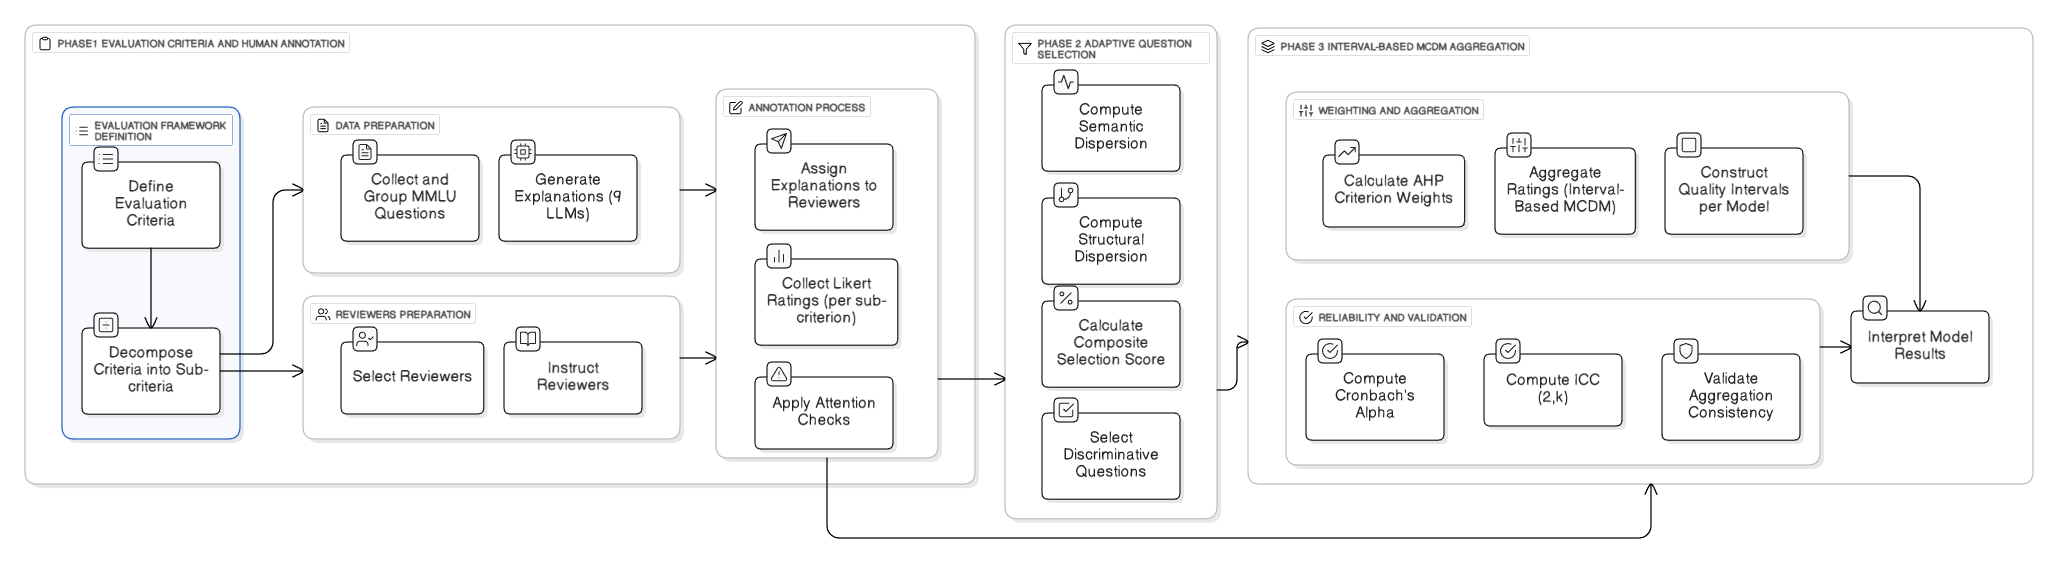
\includegraphics[width=0.95\textwidth]{figures/diagram.png}
  \caption{Overview of the three-stage evaluation pipeline: (A) criteria and
    AHP weighting, (B) Question selection via dispersion scoring, and
    (C) interval-based aggregation of Likert ratings.
    Produced by \texttt{code/LLMsAnswers.ipynb}.}
  \label{fig:pipeline}
\end{figure}

% ---------------------------------------------------------------
\section{Stage A: Evaluation Criteria and AHP Weighting}
\label{sec:meth-criteria}

\subsection{Evaluation Dimensions}
\label{subsec:meth-dimensions}

Following \citet{hoffman2019metrics}, explanation quality is assessed using four
criteria, each decomposed into two sub-criteria, yielding eight measurable
sub-dimensions in total. Satisfaction was considered as a potential fifth criterion
but was excluded because it introduces redundancy when the remaining four criteria
are already present; methodologically, its inclusion degrades AHP consistency ratios
without adding discriminative power.

\begin{description}
  \item[Understandability (C1)] Captures how easily a reviewer can make sense of
    the explanation. Its sub-criteria are:
    \begin{itemize}
      \item \textbf{S1.1 — Clarity:} How clearly the model's workings are described.
      \item \textbf{S1.2 — Ease of Following:} How easily the reviewer can trace the
        reasoning sequence.
    \end{itemize}

  \item[Completeness (C2)] Captures the scope and depth of the explanation.
    \begin{itemize}
      \item \textbf{S2.1 — Coverage:} Whether all relevant factors are addressed.
      \item \textbf{S2.2 — Reasoning Depth:} How well the explanation describes how
        results are produced.
    \end{itemize}

  \item[Usefulness (C3)] Captures the explanation's practical value.
    \begin{itemize}
      \item \textbf{S3.1 — Goal Support:} How much the explanation helps a reviewer
        achieve intended outcomes.
      \item \textbf{S3.2 — Decision-Making / Error Prevention:} How well it helps
        reviewers judge reliability or avoid mistakes.
    \end{itemize}

  \item[Trustworthiness (C4)] Evaluates whether the explanation aligns with the
    model's actual behaviour.
    \begin{itemize}
      \item \textbf{S4.1 — Reliability:} The accuracy and consistency of the
        explanation.
      \item \textbf{S4.2 — Alignment and Safety:} Whether the explanation conveys
        when outputs are valid or should be treated with caution.
    \end{itemize}
\end{description}

\subsection{Analytic Hierarchy Process}
\label{subsec:meth-ahp}

Criterion weights are derived via AHP \citep{saaty1987ahp}. Reviewers provide
pairwise importance judgments using Saaty's 9-point scale, producing a $4 \times 4$
matrix of major-criteria comparisons and four $2 \times 2$ sub-criteria matrices.
The principal eigenvector of each matrix yields local priority weights; global
weights are obtained by multiplying local weights down the hierarchy.

Consistency is verified through the Consistency Ratio:
\begin{equation}
  \mathrm{CR} = \frac{\mathrm{CI}}{\mathrm{RI}}, \quad
  \mathrm{CI} = \frac{\lambda_{\max} - n}{n - 1},
  \label{eq:cr}
\end{equation}
where $\lambda_{\max}$ is the principal eigenvalue, $n$ is the matrix dimension, and
$\mathrm{RI}$ is the average random consistency index for matrices of that size. A
matrix is accepted when $\mathrm{CR} < 0.10$ \citep{saaty1987ahp}.

Judges whose CR exceeds this threshold are excluded from the weight-derivation step
but retain their Likert ratings for the model evaluation step. Among the ten judges
who provided comparison matrices, four (J1, J2, J3, J8) satisfied the consistency
requirement. The retained weights are aggregated as a CR-weighted geometric mean
across consistent judges, so that judges with lower CR values exert proportionally
more influence.

The AHP computations are implemented in \texttt{code/Priorities\_Calculations.ipynb}.

% ---------------------------------------------------------------
\section{Stage B: Question Selection}
\label{sec:meth-qselect}

\subsection{Dataset}
\label{subsec:meth-dataset}

The MMLU benchmark \citep{hendrycks2021mmlu} is a large test set covering many
academic subjects through multiple-choice questions. The Economics subset contains
140 items. A full evaluation of this set is infeasible: with 140 questions, 9 models,
and 3 independent ratings per model output, the total reaches 3{,}780 judgments.
This workload exceeds the capacity of the reviewer pool, so a compact but informative
subset is required.

Questions are categorised into five reasoning types following \citet{hendrycks2021mmlu}:
Academic Knowledge, Procedural Knowledge, Problem Solving Ability, Qualitative
Reasoning, and Quantitative Reasoning.

\subsection{Representation}
\label{subsec:meth-embeddings}

For each question, the causal reasoning steps produced by all nine models are merged
into a single text span. Normalised sentence embeddings are produced using a
lightweight transformer encoder \citep{muennighoff2023mteb}, representing each
explanation as a vector:
\begin{equation}
  \mathbf{v}_{i} \in \mathbb{R}^{d}, \quad i = 1, \ldots, M,
  \label{eq:embedding}
\end{equation}
where $d$ is the embedding dimensionality and $M = 9$ is the number of models.

\subsection{Semantic Dispersion}
\label{subsec:meth-semantic}

Semantic dispersion measures how far model explanations diverge in meaning. The
centroid of embeddings for question $q$ is:
\begin{equation}
  \bar{\mathbf{v}}_{q} = \frac{1}{M}\sum_{i=1}^{M}\mathbf{v}_{i}, \qquad
  \text{normalised to unit length.}
  \label{eq:centroid}
\end{equation}

Semantic dispersion is the mean cosine distance from the centroid:
\begin{equation}
  D_{\mathrm{sem}}(q) = \frac{1}{M}\sum_{i=1}^{M}
    \left(1 - \frac{\mathbf{v}_{i}\cdot\bar{\mathbf{v}}_{q}}
                   {|\mathbf{v}_{i}||\bar{\mathbf{v}}_{q}|}\right).
  \label{eq:dsem}
\end{equation}

\subsection{Structural Dispersion}
\label{subsec:meth-structural}

Semantic distance alone does not capture differences in the logical structure of
explanations. Structural dispersion is therefore computed using normalised Jaccard
distance across the sets of causal steps extracted from each model output
\citep{wahyuningsih2021text, rinjeni2024matching}:
\begin{equation}
  d_J(R_{i,q}, R_{j,q}) = 1 - \frac{|R_{i,q} \cap R_{j,q}|}{|R_{i,q} \cup R_{j,q}|},
  \label{eq:jaccard}
\end{equation}
where $R_{i,q}$ and $R_{j,q}$ are the reasoning-step sets of models $i$ and $j$ for
question $q$. The structural dispersion is the mean pairwise distance:
\begin{equation}
  D_{\mathrm{struct}}(q) = \frac{2}{M(M-1)}\sum_{1 \le i < j \le M}d_J(R_{i,q},R_{j,q}).
  \label{eq:dstruct}
\end{equation}

\subsection{MAD-Style Selection}
\label{subsec:meth-mad}

The combined dispersion score is formed as a linear combination:
\begin{equation}
  D(q) = \alpha \, D_{\mathrm{sem}}(q) + (1-\alpha)\, D_{\mathrm{struct}}(q),
  \label{eq:combined}
\end{equation}
where $\alpha = 0.5$ trades off semantic and structural dispersion equally.

To avoid selecting redundant questions that are semantically similar to each other,
a diversity bonus is added following the Maximum Differentiation (MAD) competition
principle \citep{wang2008mad, feng2025sample}. At each iteration, the selection score
for a candidate question $q$, given the set of already-selected questions $S_{\mathrm{sel}}$,
is:
\begin{equation}
  \mathrm{Score}(q) = D(q) + \beta \cdot
    \max_{s \in S_{\mathrm{sel}}}\left(1 - \frac{\bar{\mathbf{v}}_{q}\cdot\bar{\mathbf{v}}_{s}}
                                               {|\bar{\mathbf{v}}_{q}||\bar{\mathbf{v}}_{s}|}\right),
  \label{eq:madscore}
\end{equation}
where $\beta = 0.3$ controls the weight of the diversity term. The question with the
highest score is selected, the set $S_{\mathrm{sel}}$ is updated, and the process
repeats until $K = 12$ questions are chosen.

This procedure yields a compact set of 12 questions that show high model disagreement
in both semantic and structural terms and cover distinct regions of the explanation
space, maximising the utility of the limited reviewer budget \citep{feng2025sample}.

The selection procedure is implemented in
\texttt{code/LLMsAnswers.ipynb} (model querying and response collection) and
\texttt{code/E2\_AHP\_CSV\_AND\_GRAPHS.ipynb} (dispersion computation and question
selection).

% ---------------------------------------------------------------
\section{Stage C: Interval-Based Aggregation}
\label{sec:meth-aggregation}

\subsection{Data Collection and Rating Protocol}
\label{subsec:meth-collection}

Nine graduate students with economics backgrounds were recruited from Tunis Business
School as reviewers. Data collection was conducted via a structured online survey in
December 2025. Each reviewer rated a randomised subset of 36 explanation instances
drawn from the pool of $12 \times 9 = 108$ instances, ensuring every instance
received exactly three independent assessments. Ratings were given on a 5-point
Likert scale across all eight sub-criteria, yielding $108 \times 3 \times 8 = 2{,}592$
judgments in total. Attention-check trials were interleaved throughout to ensure
response quality \citep{roth2024attention}, and presentation order was fully
randomised within subjects to mitigate ordering effects \citep{beck2024order}.

\subsection{Interval Representation}
\label{subsec:meth-interval}

For each model $m$ and sub-criterion $j$, the Likert ratings collected from the
three raters are represented through their interquartile range:
\begin{equation}
  I_{mj} = [Q_1^{mj},\; Q_3^{mj}],
  \label{eq:iqr}
\end{equation}
where $Q_1$ and $Q_3$ denote the first and third quartiles of the rating
distribution. Unlike simple averaging, the IQR makes both consensus and divergence
visible without being distorted by extreme values, treating reviewer disagreement
as meaningful signal rather than noise \citep{hayes2007answering}.

\subsection{Weighted Aggregation}
\label{subsec:meth-aggregation2}

Sub-criterion intervals are aggregated into criterion-level intervals via weighted
summation using AHP-derived weights $W_k$ (criterion level) and $w_{kj}$
(sub-criterion level within criterion $k$):
\begin{equation}
  T_m = \left[\sum_{k}\sum_{j} W_k \cdot w_{kj} \cdot Q_1^{mj},\;\;
              \sum_{k}\sum_{j} W_k \cdot w_{kj} \cdot Q_3^{mj}\right].
  \label{eq:aggregate}
\end{equation}
This yields a final quality interval $T_m = [T_{Q1}^m, T_{Q3}^m]$ for each model.

Models are ranked by the lower bound $T_{Q1}^m$ as the primary criterion, with
the midpoint of the interval serving as a tiebreaker. A wider interval indicates
greater reviewer disagreement, interpreted as evidence of reasoning instability in
the underlying model.

\subsection{Reliability Analysis}
\label{subsec:meth-reliability}

Aggregation validity requires $\mathrm{Cronbach's}\ \alpha \ge 0.70$ and
$\mathrm{ICC}(2, k) \ge 0.60$ \citep{hayes2007answering}. Three complementary
analyses are applied:

\begin{itemize}
  \item \textbf{Bootstrapped confidence intervals:} Repeated resampling is used to
    estimate the stability of model scores when standard assumptions may not hold
    \citep{zapf2016measuring}.
  \item \textbf{Inter-rater reliability:} Intraclass Correlation Coefficient
    $\mathrm{ICC}(2,k)$ and Krippendorff's $\alpha$ (interval) are computed to
    quantify agreement across reviewers \citep{saal1980rating, hayes2007answering}.
  \item \textbf{Effect-size analysis:} Cohen's $d$ and Hedges' $g$ quantify the
    magnitude of score differences between the top and bottom models
    \citep{steiger2004beyond}.
\end{itemize}

All aggregation and reliability computations are implemented in
\texttt{code/E2\_AHP\_CSV\_AND\_GRAPHS.ipynb}.
